\setcounter{secnumdepth}{3}

\chapter{Compiling OTB from source}
\label{chapter:Installation}
\index{Installation}

There are two ways to install OTB library on your system: installing from a binary distribution or compiling from sources. 
You can find information about the installation of binary packages for OTB and Monteverdi in the OTB-Cookbook.

This chapter covers compilation of OTB library from source. Note that it covers
also the compilation of Monteverdi which is integrated as an OTB module since
version 5.8.

OTB has been developed and tested across different combinations of operating
systems, compilers, and hardware platforms including Windows, Linux and Mac OSX.
It is known to work with the following compilers in 32/64 bit:
\begin{itemize}
\item Visual Studio 2015 on Windows
\item GCC 4.x,5.x or CLang 3.x on GNU/Linux
\item AppleClang on Mac~OS~X (10.8 or higher)
\end{itemize}

\index{CMake}
The challenge of supporting OTB across platforms has been solved through the use of CMake, a cross-platform, open-source
build system. CMake is used to control the software compilation process using simple platform and compiler independent
configuration files.  CMake generates native makefiles and workspaces that can be used in the compiler environment of
your choice. CMake is quite sophisticated: it supports complex environments requiring system configuration, compiler
feature testing, and code generation.

CMake supports several generators to produce the compilation scripts, dependending on the platform and compiler. It can use :
\begin{itemize}
\item Makefiles for Unix systems
\item Visual Studio workspaces for Windows
\item NMake Makefiles for Windows
\item Ninja scripts
\item and many more ...
\end{itemize}
The information used by CMake is provided by \code{CMakeLists.txt} files that
are present in every directory of the OTB source tree. These files contain information that the user provides to CMake
at configuration time. Typical information includes paths to utilities in the system and the selection of software
options specified by the user.

There are (at least) two ways to use CMake :
\begin{itemize}
\item Using the command \texttt{ccmake} (on Unix) or \texttt{cmake-gui} (on Windows): 
it provides an interactive mode in which you iteratively select
options and configure according to these options. The iteration
proceeds until no more options remain to be selected. At this point, a
generation step produces the appropriate build files for your
configuration. This is the easiest way to start.
\item Using the command \texttt{cmake} : it is a non-interactive polyvalent tool designed for scripting. It can run both \textit{configure} and \textit{generate} steps.
\end{itemize}

As shown in figure \ref{fig:CMakeGUI}, CMake has a different interfaces according to your system.
Refer to section~\ref{sec:compiling-linux} for Linux and Mac~OS~X build instructions
and \ref{sec:compiling-windows} for Windows.

\begin{figure}[tpb]
\centering
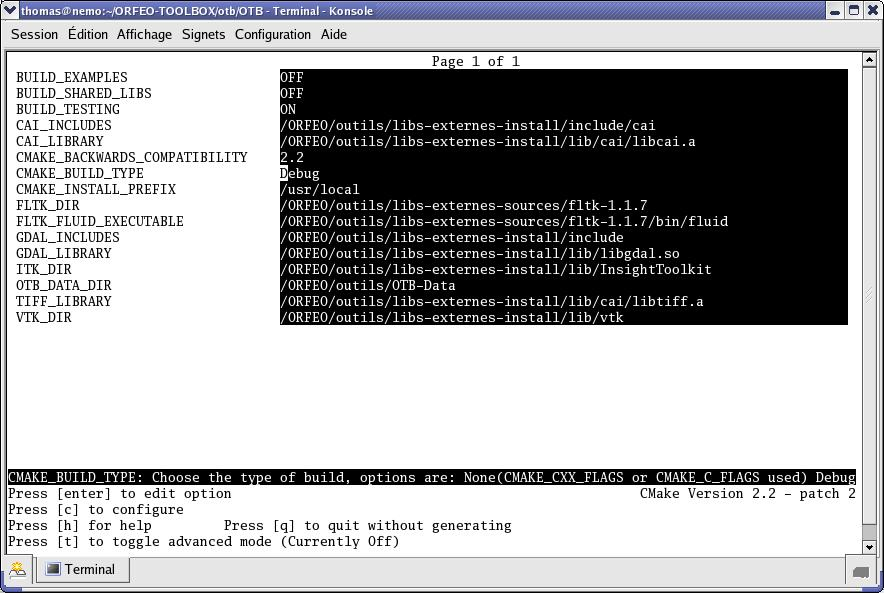
\includegraphics[width=0.8\textwidth]{ccmakeScreenShot.eps}
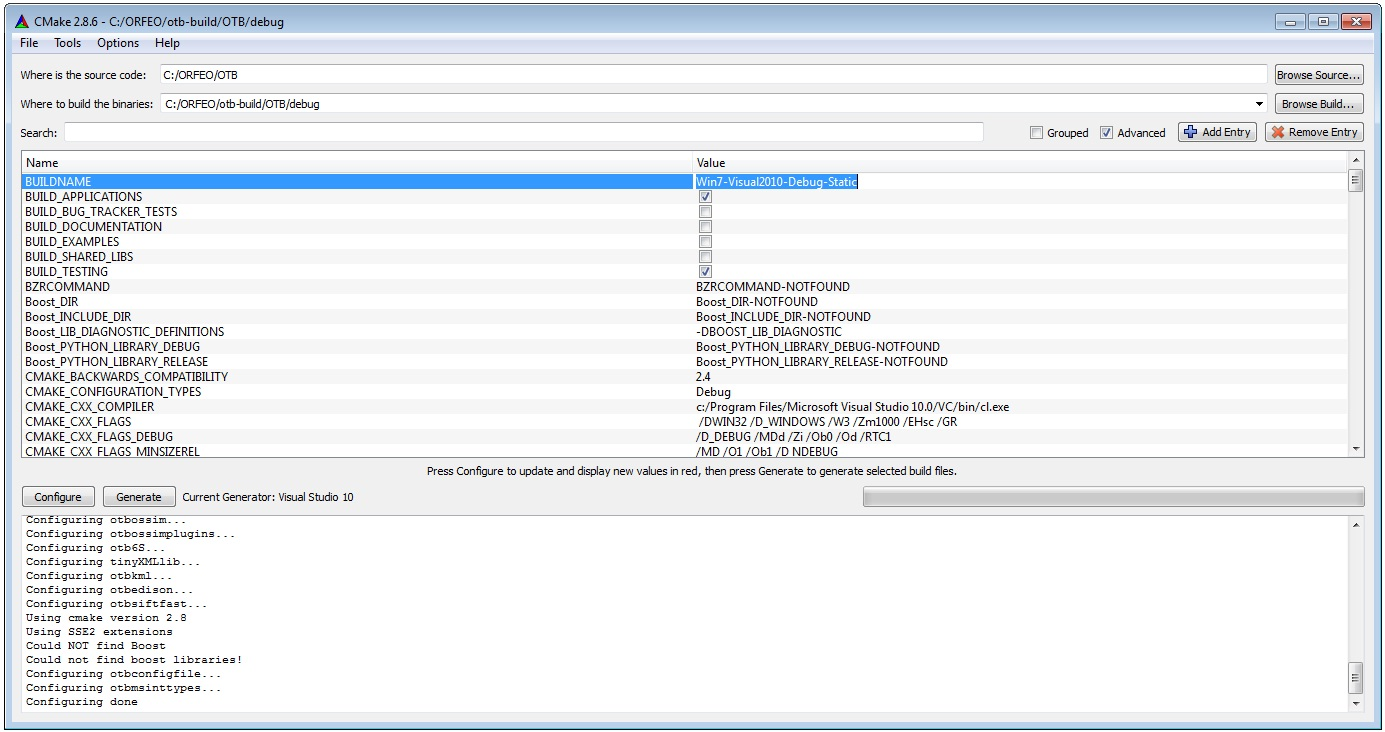
\includegraphics[width=0.8\textwidth]{CMakeSetupScreenShot.eps}
\itkcaption[Cmake user interface]{CMake interface. Top) \texttt{ccmake}, the UNIX
version based on \texttt{curses}. Bottom) \texttt{CMakeSetup}, the MS-Windows
version based on MFC.}
\label{fig:CMakeGUI}
\end{figure}

For more information on CMake, check :
\begin{center}
\url{http://www.cmake.org}
\end{center}

\index{Dependencies}
OTB depends on a number of external libraries.  Some are mandatory, meaning that
OTB cannot be compiled without them, while others (the majority) are optional
and can be activated or not during the build process.
See table \ref{tab:otb-dependencies} for the full list of dependencies.
\begin{center}
\begin{tiny}
\begin{table}[!htbp]
\begin{tabular}{|p{0.15\textwidth}|p{0.45\textwidth}|p{0.1\textwidth}|p{0.1\textwidth}|}
\hline
\textbf{Library} & \textbf{Web site} & \textbf{Mandatory} & \textbf{Minimum version} \\
\hline
\textbf{ITK} & \url{http://www.itk.org} & yes & 4.6.0 \\
\hline
\textbf{GDAL} & \url{http://www.gdal.org} & yes & 1.10 \\
\hline
\textbf{OSSIM} & \url{http://www.ossim.org} & yes & 1.8.20-3 \\
\hline
\textbf{libgeotiff} & \url{http://trac.osgeo.org/geotiff/} & yes & - \\
\hline
\textbf{boost} & \url{http://www.boost.org} & yes & - \\
\hline
\textbf{openthreads} & \url{http://www.openscenegraph.org} & yes & - \\
\hline
\textbf{tinyXML} & \url{http://www.grinninglizard.com/tinyxml} & yes & - \\
\hline
\textbf{6S} & \url{http://6s.ltdri.org} & no & - \\
\hline
\textbf{Curl} & \url{http://www.curl.haxx.se} & no  & - \\
\hline
\textbf{FFTW} & \url{http://www.fftw.org} & no  & - \\
\hline
\textbf{GLEW} & \url{http://glew.sourceforge.net/} & no  & - \\
\hline
\textbf{GLFW} & \url{http://www.glfw.org/} & no  & 3 \\
\hline
\textbf{GLUT} & \url{https://www.opengl.org/resources/libraries/glut/} & no  & - \\
\hline
\textbf{libKML} & \url{https://github.com/google/libkml} & no  & 1.2 \\
\hline
\textbf{libSVM} & \url{http://www.csie.ntu.edu.tw/~cjlin/libsvm} & no  & 2.0 \\
\hline
\textbf{Mapnik} & \url{http://www.mapnik.org} & no  & 2.x \\
\hline
\textbf{MPI} & \url{https://www.open-mpi.org/} & no  & - \\
\hline
\textbf{MuParser} & \url{http://www.muparser.sourceforge.net} & no  & - \\
\hline
\textbf{MuParserX} & \url{http://muparserx.beltoforion.de} & no  & 4.0.7 \\
\hline
\textbf{OpenCV} & \url{http://opencv.org} & no  & 2 \\
\hline
\textbf{OPENGL} & \url{https://www.opengl.org/} & no  & - \\
\hline
\textbf{Qt} & \url{http://qt-project.org} & no  & 4 \\
\hline
\textbf{QWT} & \url{http://qwt.sourceforge.net} & no  & 5 \\
\hline
\textbf{Shark} & \url{http://image.diku.dk/shark/} & no & 3.1 \\
\hline
\textbf{SiftFast} & \url{http://libsift.sourceforge.net} & no  & - \\
\hline
\textbf{SPTW} & \url{https://github.com/kornholi/sptw.git} & no  & - \\
\hline

\end{tabular}
\caption{External libraries used in OTB.}
\label{tab:otb-dependencies}
\end{table}
\end{tiny}
\end{center}

\section{Linux and Mac OS X}
\label{sec:compiling-linux}

\subsection{Setting up the build environment}

The first thing to do is to create a directory for working with OTB.
This guide will use \texttt{$\sim$/OTB} but you are free to choose something else.
In this directory, there will be three locations:
\begin{itemize}
\item \texttt{$\sim$/OTB/otb} for the source file obtained from the git repository
\item \texttt{$\sim$/OTB/build} for the intermediate build objects, CMake specific files, libraries and binaries.
\item \texttt{$\sim$/OTB/install}, the installation directory for OTB once it is built.
A system location (\texttt{/usr/local} for example) can also be used, but installing locally is more flexible and does
not require root access.
\end{itemize}
To setup this structure, the following commands can be used:
\begin{verbatim}
$ mkdir ~/OTB
$ cd ~/OTB
$ git clone https://git@git.orfeo-toolbox.org/git/otb.git
$ mkdir build
$ mkdir install
\end{verbatim}

The OTB project uses a git branching model where \texttt{develop} is the current development version.
It contains the latest patches and represents the work in progress towards the next release.
For more information on OTB and git, including how to decide which branch to want to compile, please see the
OTB wiki page at \url{http://wiki.orfeo-toolbox.org/index.php/Git}.

Checkout the relevant branch now:
\begin{verbatim}
$ cd ~/OTB/otb
$ git checkout develop
\end{verbatim}

Now you must decide which build method you will use.
There are two ways of compiling OTB from sources, depending on how you want to manage dependencies.
Both methods rely on CMake.
\begin{itemize}
\item SuperBuild (go to section~\ref{sec:installation-linux-superbuild}). All OTB dependencies are automatically downloaded and compiled.
This method is the easiest to use and provides a complete OTB with minimal effort.
\item Normal build (go to section~\ref{sec:installation-linux-normalbuild}). OTB dependencies must already be compiled and available on your system.
This method requires more work but provides more flexibility.
\end{itemize}
If you do not know which method to use and just want to compile OTB with all its modules, use SuperBuild.

\begin{center}
\begin{tiny}
\begin{table}[!htbp]
\begin{tabular}{p{0.35\textwidth}p{0.65\textwidth}}
\hline
\textbf{CMake variable} & \textbf{Value} \\
\hline
\texttt{CMAKE\_INSTALL\_PREFIX}         & Installation directory, target for \texttt{make install} \\
\texttt{BUILD\_EXAMPLES}                & Activate compilation of OTB examples \\
\texttt{BUILD\_TESTING}                 & Activate compilation of the tests \\
\texttt{OTB\_BUILD\_DEFAULT\_MODULES}   & Activate all usual modules, required to build the examples \\
\texttt{OTB\_USE\_\textit{XXX}}         & Activate module \textit{XXX} \\
\texttt{OTBGroup\_\textit{XXX}}         & Enable modules in the group \textit{XXX} \\
\texttt{OTB\_DATA\_ROOT}                & otb-data repository \\
\texttt{OTB\_WRAP\_PYTHON}              & Enable Python wrapper \\
\texttt{OTB\_WRAP\_JAVA}                & Enable Java wrapper \\

\hline
\multicolumn{2}{l}{\small \textbf{SuperBuild only}} \\ 
\texttt{DOWNLOAD\_LOCATION}             & Location to download dependencies \\
\texttt{USE\_SYSTEM\_\textit{XXX}}      & Use the system's \textit{XXX} library \\

\hline
\end{tabular}
\caption{Important CMake configuration variables in OTB}
\label{tab:installation-cmake-variables}
\end{table}
\end{tiny}
\end{center}

\subsection{SuperBuild: Build OTB and all dependencies}
\label{sec:installation-linux-superbuild}

The SuperBuild is a way of compiling dependencies to a project just before you
build the project. Thanks to CMake and its ExternalProject module, it is
possible to download a source archive, configure and compile it when building
the main project. This feature has been used in other CMake-based projects (ITK,
Slicer, ParaView,...).  In OTB, the SuperBuild is implemented with no impact on
the library sources : the sources for SuperBuild are located in the
'OTB/SuperBuild' subdirectory. It is made of CMake scripts and source patches
that allow to compile all the dependencies necessary for OTB. Once all the
dependencies are compiled and installed, the OTB library is built using those
dependencies.

OTB's compilation is customized by specifying configuration variables.  The most
important configuration variables are shown in
table~\ref{tab:installation-cmake-variables}.  The simplest way to provide
configuration variables is via the command line \texttt{-D} option:
\begin{verbatim}
$ cd ~/OTB/build
$ cmake -D CMAKE_INSTALL_PREFIX=~/OTB/install ../otb/SuperBuild
\end{verbatim}
A pre-load script can also be used with the \texttt{-C} options (see
\url{https://cmake.org/cmake/help/v3.4/manual/cmake.1.html#options}).
Another option is to set variables manually with \texttt{cmake-gui}
or \texttt{ccmake}.

Please note that the \texttt{CMAKE\_INSTALL\_PREFIX} variable is
important because the SuperBuild will install some targets during the
compilation step.  Therefore this directory will be used even if you
don't use make install target.  In fact there is no make install
target for the SuperBuild. Also note that if not specified to cmake, a
default install dir will be used, located in \texttt{../superbuild\_install}.

By default, SuperBuild will not use any of libraries installed on
system. All \texttt{USE\_SYSTEM\_\textit{XXX}} are set to FALSE. This is our
recommended way of using SuperBuild. You are however free to use a system
library if you want!. You must be very much aware of dependencies of those
libraries you use from system. For example, if libjpeg is not used from
superbuild then you should not use zlib from superbuild because zlib is a dependency of libjpeg.
Here SuperBuild will NOT set \texttt{USE\_SYSTEM\_ZLIB=FALSE}. One must re-run cmake
with \texttt{-DUSE\_SYSTEM\_ZLIB=FALSE}.
Above example of libjpeg-zlib dependency is so simple.  Imagine
the case for GDAL which depends on zlib, libjpeg, libtiff(with big tiff
support), geotiff, sqlite, curl, geos, libkml, openjpeg. This is one of the
reasons we recommend to use SuperBuild exclusively.

All dependencies are configured and built in a way that help us to get an
efficient build OTB.  So we enable geotiff (with proj4 support), openjpeg, geos
in GDAL build.

(see table~\ref{tab:installation-cmake-variables}).

SuperBuild downloads dependencies into the \texttt{DOWNLOAD\_LOCATION}
directory, which will be
\texttt{$\sim$/OTB/build/Downloads} in our example.
Dependencies can be downloaded manually into this directory before the
compilation step.  This can be useful if you wish to bypass a proxy, intend to
compile OTB without an internet connection, or other network constraint. You can
find an archive with sources of all our dependencies on the Orfeo ToolBox
website (pick the 'SuperBuild-archives' corresponding to the OTB version you
want to build) :
\begin{center}
\url{https://www.orfeo-toolbox.org/packages}
\end{center}

Qt library: Unlike other dependencies building Qt4 on all platform is not trivial task but
OTB SuperBuild makes best effort to make it easier for you. So there is still
some additional package installation, one has to do as a pre-requistie for SuperBuild
On a GNU/Linux you must have Qt X11 dependencies installed.
See Qt 4.8 documentation for list of packages that needs to be installed
before starting superbuild. http://doc.qt.io/qt-4.8/requirements-x11.html
For a debian 8.1 systeme, I installed all Qt4 dependencies with below 'apt-get install'
\texttt{apt-get install libx11-dev libxext-dev libxt-dev libxi-dev libxrandr-dev libgl-dev libglu-dev}

You can also deactivate QT4 and skip this by passing \texttt{-DOTB\_USE\_QT4=OFF} to cmake.
This will give you OTB install without monteverdi, mapla and gui application launchers.

For Mac OSX you need to install XCode and Windows 7,8.1,10 requires MSVC 2015 or higher.

You are now ready to compile OTB!
Simply use the make command (other targets can be generated with CMake's \texttt{-G} option):
\begin{verbatim}
$ cd ~/OTB/build
$ make
\end{verbatim}

Applications will be located in the \texttt{bin/} directory
in CMAKE\_INSTALL\_PREFIX
directory, which in our case is \texttt{~/OTB/install/bin/}. For example:
\begin{verbatim}
~/OTB/install/bin/otbcli_ExtractROI
\end{verbatim}
will launch the command line version of the \textbf{ExtractROI} application,
while:
\begin{verbatim}
./OTB/install/bin/otbgui_ExtractROI
\end{verbatim}
will launch the graphical version.

To be able to use your OTB build from everywhere, we recommend the following.
First, add \texttt{bin/} directory to your PATH for easy access:
\begin{verbatim}
export PATH=$PATH:~/OTB/install/bin
\end{verbatim}

Second, add the \texttt{lib/} directory to your LD\_LIBRARY\_PATH:
\begin{verbatim}
export LD_LIBRARY_PATH=~/OTB/install/lib:$LD_LIBRARY_PATH
\end{verbatim}

Monteverdi is integrated as an OTB module since release 5.8 and it is compiled
by the SuperBuild (as long as GLEW, GLUT, OPENGL, Qt and QWT modules are
activated).

To use OTB applications from within Monteverdi you will need to define the
OTB\_APPLICATION\_PATH environment variable.
\begin{verbatim}
export OTB_APPLICATION_PATH=~/OTB/install/lib/otb/applications
monteverdi
\end{verbatim}

A wiki page detailing the status of SuperBuild on various platforms is also available here:
\url{http://wiki.orfeo-toolbox.org/index.php/SuperBuild}.

\subsection{Normal build: Build only OTB}
\label{sec:installation-linux-normalbuild}

Once all OTB dependencies are availables on your system, use CMake to generate a Makefile:
\begin{verbatim}
$ cd ~/OTB/build
$ cmake -C configuration.cmake ../otb
\end{verbatim}
The script \texttt{configuration.cmake} needs to contain dependencies location
if CMake cannot find them automatically.  This can be done with
the \texttt{\textit{XXX}\_DIR} variables containing the directories which
contain the FindXXX.cmake scripts, or with the \texttt{\textit{XXX}\_INCLUDEDIR}
and \texttt{\textit{XXX}\_LIBRARY} variables.

Additionally, decide which module you wish to enable, together with tests and
examples.  Refer to table~\ref{tab:installation-cmake-variables} for the list of
CMake variables.

Since OTB is modularized, it is possible to only build some modules instead of
the whole set.  To deactivate a module (and the ones that depend on it) switch
off the CMake variable OTB\_BUILD\_DEFAULT\_MODULES, configure, and then switch
off each \texttt{Module\_module\_name} variable.  To provide an overview on how
things work, the option \texttt{COMPONENTS} of the CMake command find\_package
is used in order to only load the requested modules.  This module-specific list
prevent CMake from performing a blind search; it is also a convienent way to
monitor the dependencies of each module.
\begin{verbatim}
find_package(OTB COMPONENTS OTBCommon OTBTransform [...])
\end{verbatim} 

Some of the OTB capabilities are considered as optional, and you can deactivate
the related modules thanks to a set of CMake variables starting
with \texttt{OTB\_USE\_\textit{XXX}}.  Table~\ref{tab:optional} shows which
modules are associated to these variables. It is very important to notice that
these variable override the variable OTB\_BUILD\_DEFAULT\_MODULES.

You are now ready to compile OTB!  Simply use the make command (other targets
can be generated with CMake's \texttt{-G} option):
\begin{verbatim}
$ make
\end{verbatim}

The installation target will copy the binaries and libraries to the installation
location:
\begin{verbatim}
$ make install
\end{verbatim}

\begin{center}
\begin{tiny}
\begin{table}[!htbp]
\begin{tabular}{|l|l|p{0.52\textwidth}|}
\hline
\textbf{CMake variable} & \textbf{3rd party module} & \textbf{Modules depending on it} \\
\hline
\textbf{OTB\_USE\_LIBKML} & OTBlibkml & OTBKMZWriter OTBIOKML OTBAppKMZ \\
\hline
\textbf{OTB\_USE\_QT4} & OTBQt4 & OTBQtWidget \\
\hline
\textbf{OTB\_USE\_OPENCV} & OTBOpenCV & \\
\hline
\textbf{OTB\_USE\_MUPARSERX} & OTBMuParserX & OTBMathParserX OTBAppMathParserX \\
\hline
\textbf{OTB\_USE\_CURL} & OTBCurl & \\
\hline
\textbf{OTB\_USE\_MUPARSER} & OTBMuParser & OTBMathParser OTBDempsterShafer OTBAppClassification OTBAppMathParser OTBAppStereo OTBAppProjection OTBAppSegmentation OTBAppClassification OTBRoadExtraction OTBRCC8 OTBCCOBIA OTBAppSegmentation OTBMeanShift OTBAppSegmentation OTBMeanShift OTBAppSegmentation \\
\hline
\textbf{OTB\_USE\_LIBSVM} & OTBLibSVM & OTBSVMLearning \\
\hline
\textbf{OTB\_USE\_MAPNIK} & OTBMapnik & OTBVectorDataRendering \\
\hline
\textbf{OTB\_USE\_6S} & OTB6S & OTBOpticalCalibration OTBAppOpticalCalibration OTBSimulation \\
\hline
\textbf{OTB\_USE\_SIFTFAST} & OTBSiftFast & \\
\hline
\end{tabular}
\caption{Third parties and related modules.}
\label{tab:optional}
\end{table}
\end{tiny}
\end{center}

\section{Windows}
\label{sec:compiling-windows}

Everything that is needed for OTB development on Windows, including compiling from source, is covered in details on the OTB wiki at:
\begin{center}
\url{http://wiki.orfeo-toolbox.org/index.php/OTB_development_on_Windows}
\end{center}

\section{Known issues}
\label{sec:knownissues}

\begin{itemize}
\item  openjpeg/ITK 
\end{itemize}

It is important to know that the OpenJpeg library doesn't support name mangling since version 2.0. 
As a consequence, if other libraries linked by your project already contain OpenJpeg, there may be a symbol conflict at run-time. 
For instance, this was observed with OTB build on a recent ITK version (ver. 4). 
The ITK library already had a version of OpenJpeg in libitkopenjpeg-*.so, which contained the OpenJpeg symbols un-wrapped.
These symbols were also loaded by the GDAL driver but only the first ones were used, which caused a crash. 

Hopefully, thanks to the modular architecture of ITK, the library libitkopenjpeg-*.so is not imported anymore inside OTB.
However the OpenJPEG headers may be present in ITK include directory. As the current architecture doesn't allow to tune 
include order between modules, the OpenJPEG header from ITK can be included before your own OpenJPEG install. There are
two ways to avoid this situation :
\begin{itemize}
\item Use an ITK without GDCM nor ITKReview (only these modules depend on OpenJPEG)
\item Hide the header openjpeg.h in the ITK include directory.
\end{itemize}

More information can be found here : \url{http://wiki.orfeo-toolbox.org/index.php/JPEG2000_with_GDAL_OpenJpeg_plugin}

\begin{itemize}
\item  libkml / Ubuntu 12.04 
\end{itemize}

Another issue is related to the official package of libkml under Ubuntu 12.4.
Until this problem is addressed, users of this plateform should disable the option OTB\_USE\_KML, so that OTB won't be built with this third-party.

